\documentclass[11pt,a4paper]{article}
\usepackage[T1]{fontenc}
\usepackage[utf8]{inputenc}
\usepackage[french]{babel}
\usepackage{color}
\usepackage{graphicx}
\usepackage{float}
\usepackage{hyperref}
\author{Durand Leo, Tsamarayev Massoud, Mohamed Saandi}
\date{\today}
\begin{document}

\title{
	\color{blue}
	\textbf{Le Mans Université}\\
	\color{black}
	Licence Informatique 2ème année\\
	Module 174UP02 Rapport de Projet\\
	\textbf{For The King}\\
}

\begin{figure}[t]
\centering

\includegraphics[height=1cm]{logolemansU.png}
\hfill

\includegraphics[height=1.5cm]{logo_IC2.png}

\end{figure}

\maketitle

\newpage

\tableofcontents

\newpage

\section{Introduction}

\textbf{Contexte du projet} \\
Ce document présente le projet de développement du jeu For The King, réalisé dans le cadre de la deuxième année de licence Informatique à l'université du Mans, pendant la période de de janvier à février 2026.
L'objectif principal est la conception et l'implémentation d'un jeu vidéo en langage C, en utilisant la bibliothèque graphique SDL2 pour la gestion de l'affichage et des interactions.

\medskip

\textbf{Objectifs techniques} \\
Ce projet vise à mettre en pratique des concepts informatiques fondamentaux :
\begin{itemize}
	\item \textbf{Gestion de la mémoire} : Manipulation des pointeurs et des structures en C pour éviter toute fuite mémoire.
	\item \textbf{Architecture logicielle} : Structuration du code pour séparer la logique de jeu (moteur) du rendu graphique (SDL2).
	\item \textbf{Algorithmique} : De façon plus générale, utiliser les concepts clés vus en cours en Algorithmique 2 et Algorithmique 3.
\end{itemize}

\medskip

\textbf{Plan du rapport} \\
Nous commencerons par expliquer la conception du jeu, c'est-à-dire une présentation du jeu et de ses fonctionnalités.
Puis dans un second temps nous expliquerons comment le projet s'est organisé, en parlant du planning prévisionnel, de la répartition des tâches ainsi que des outils techniques utilisés.
Ensuite le rapport traitera du développement du jeu, et montrera comment est programmée de façon générale chaque fonctionnalité du jeu.
Enfin nous dévoilerons le bilan et les résultats de ce projet.
Une bibliographie et une annexe sont également disponibles.

\section{Conception}

La phase de conception permet de réfléchir sur, comment le jeu sera construit avant de coder. L'idée principale est de créer un système composé de plusieurs parties qui fonctionnent de manière indépendante, c'est-à-dire, chaque élément du jeu, comme la carte, les combats et l'interface utilisateur, peut être développé et testé séparément sans affecter les autres parties du jeu. Cette façon de réfléxion est basée sur trois principes simples :

\begin{itemize}
    \item \textbf{Séparation des éléments} : chaque fonctionnalité est séparée pour éviter qu'une modification ne casse pas le reste du programme (\textbf{flexible}).
    \item \textbf{Évolutivité} : la structure facilite les ajours futurs de nouveaux personnages ou de nouvelles mécaniques par exemple (\textbf{réutilisable}).
    \item \textbf{Flexibilité} : l'architecture permet une meilleure gestion de la carte générée dynamiquement (\textbf{évolutif}).
    \item \textbf{Clarté du code} : l'organisation permet de comprendre rapidement comment le programme fonctionne sans perdre du temps (\textbf{lisible} et \textbf{maintenable}).
\end{itemize}

Cela permet donc de maintenir et que les mécaniques de gameplay pourront être modifiées tout au long du développement du jeu.

\subsection{Présentation du jeu}

\textbf{Présentation et principe du jeu}

\noindent\textit{For The King} est un jeu de rôle (RPG) et d'aventure intégrant des mécaniques de combat au tour par tour. 
Le joueur est placé dans le royaume, plongé dans le chaos. 
L'objetic est de préparer le héros à un affrontement contre le boss final pour restaurer la paix dans le royaume. 

Le gameplay repose sur une boucle de progression stratégique autour de trois axes : 

\begin{itemize}
	\item \textbf{L'exploration et les quêtes} : Le joueur parcourt la carte pour découvrir des campements, des sanctuaires et remplir des objectifs secondaires.
	\item \textbf{Le combat au tour par tour} : Les affrontements opposent le personnage aux diffrérents monstres. Chaque tour permet de choisir entre une attaque légère (précise mais moins puissante) et une attaque lourde (dégâts élevés mais probabilité d'échec élevés).
	\item \textbf{La gestion des ressources} : L'élimination des ennemis octroie de l'or et des objets de soin. L'or est une ressource essentielle permettant de se reposer afin de regagner de la vie ou d'acheter des kits de soin dans les campements.
\end{itemize} 

\medskip

\textbf{Mécaniques de progression} 

\noindent La progression du personnage est nécessaire pour vaincre le boss final. 
Le joueur peut obtenir des bénédictions via les sanctuaires. 
Les sanctuaires sont rares c'est pourquoi ils offrent des bonus de statistiques permanents. 
Chaque sanctuaire ne peut être utilisé qu'une seule fois, ce qui demande au joueur de faire des choix stratégiques durant son aventure.
De plus, le personnage peut gagner de l'expérience en gagnant des combats contre des monstres. En gagnant de l'expérience, 
le personnage peut monter de niveau, ce qui augmente ses statistiques légèrement.

\medskip

\subsection{Fonctionnalités du jeu}

\begin{table}[H]
\begin{tabular}{|l|c|}
\hline
Fonctionnalité & Explication \\
\hline
Génération aléatoire de la carte & Utilisation de l'algorithme Perlin Noise. \\
Personnage & Chaque personnage a une classe et des attributs. \\
Inventaire & Chaque personnage a un inventaire qui contient des objets. \\
Objet & On peut obtenir des objets en tuant des monstres. \\
Exemples d'objets & Kits de soins et pièces d'or. \\
Utilisation d'un objet & On peut utiliser tous les objets. \\
Interaction avec monstre & Cliquer la case du monstre sur la carte. \\
Options du combat & On peut soit fuir, soit attaquer. \\
Déroulement du combat & Tour par tour, commence par le personnage joueur. \\
Attaques possibles & Lourde ou légère. \\
Obstacles sur la carte & Montagnes, cactus, arbres etc. \\
Bâtiments sur la carte & Campement qui sert à regagner des PVs. \\
Sanctuaires sur la carte & Donnent un bonus si découverts et validés. \\
Expérience & Gagner un combat rapporte de l'EXP. \\
Niveau & Monter en niveau améliore les statistiques. \\
Quêtes & Finir les quêtes pour avoir des récompenses. \\
\hline
\end{tabular}
\label{tab_taches}
\caption{Ceci est un tableau présentant les différentes fonctionnalités du jeu et une explication.}
\end{table}

\section{Organisation du projet}

\subsection{Planning prévisionnel}

Pour planifier les tâches, nous avons utilisé un outil spécifique : les diagrammes de Gantt.
Cet outil nous a permis de créer un planning prévisionnel au début du projet, ainsi qu'un planning réel à la fin du projet.
Cela nous a permis de comparer les deux pour voir si on avait respecté le planning prévisionnel initial.

\begin{enumerate} 
	\item Dans un premier temps, nous avons commencé par la phase d'initialisation, qui consiste notamment en la mise en place du dépôt GitHub ainsi que l'installation des librairies nécessaires comme SDL2. 
	\item Puis dans un second temps, la phase de préparation a consisté à définir les bases du projet: les règles du jeu, les quêtes, les combats, la structure de la carte et les attributs des monstres et personnages. 
	\item La phase principale du projet a été le codage et les tests, qui se sont étalés sur plusieurs semaines. Nous avons travaillé sur la génération aléatoire de la carte, l'affichage avec SDL2, la création des personnages et des menus, ainsi que la programmation des systèmes de combat, des monstres, des quêtes et du boss final. Cette phase a également inclus la gestion des sauvegardes, des objets et de l'inventaire, ainsi que de nombreux tests et corrections de bugs. On remarque que certaines tâches ont pris plus de temps que prévu, notamment les fonctionnalités complexes comme les combats et la génération de la carte. 
	\item Enfin, la phase de livraison a regroupé la rédaction du rapport, la préparation de la soutenance ainsi que la documentation du code avec Doxygen. Cette phase a permis de finaliser le projet et de le rendre présentable et compréhensible de tout le monde. 
\end{enumerate}


\subsection{Répartition des tâches}

\begin{table}[H]
\begin{tabular}{|l|c|}
\hline
Tâche effectuée & Nom et prénom \\
\hline
Placement du personnage sur la carte & Durand Léo \\
Mécaniques de déplacement & Durand Léo \\
Création et utilisation des objets & Durand Léo \\
Système d'inventaire & Durand Léo \\
Sauvegarde des parties & Durand Léo \\
Affichage de la carte & Durand Léo \\
Affichage interface joueur & Durand Léo \\
Initialisation de la carte & Durand Léo \\
Tests Unitaires & Durand Léo \\
Boss final et son combat & Durand Léo \\
Musique & Durand Léo, Tsamarayev Massoud \\
Affichage des combats & Durand Léo, Tsamarayev Massoud \\
Génération de l'eau & Tsamarayev Massoud \\
Affichage hexagonal & Tsamarayev Massoud \\
Mécaniques du combat & Tsamarayev Massoud, Mohamed Saandi \\
Menu principal & Tsamarayev Massoud \\
Menu de pause & Tsamarayev Massoud \\
Graphismes & Tsamarayev Massoud, Durand Léo \\
Système de niveau & Tsamarayev Massoud \\
Placement aléatoire des monstres & Tsamarayev Massoud \\
Quêtes & Tsamarayev Massoud \\
Interactions avec les sanctuaires & Tsamarayev Massoud \\
Interactions avec les campements & Tsamarayev Massoud \\
Documentation Doxygen & Mohamed Saandi \\
Génération des biomes & Mohamed Saandi \\
Interactions avec les monstres & Mohamed Saandi \\
Gantt prévisionnel & Mohamed Saandi \\
Bruitages & Mohamed Saandi \\
Création des monstres et leur attributs & Toute l'équipe \\
Création des personnages et leur attributs & Toute l'équipe \\
Génération de la carte & Toute l'équipe \\
\hline
\end{tabular}
\label{tab_taches}
\caption{Ceci est un tableau présentant les différents étudiants qui ont travaillé sur ce projet ainsi que les tâches qu'ils ont effectué.} 
\end{table}
Tableau répartition des tâches \ref{tab_taches}

\subsection{Outils techniques utilisés}

\begin{itemize}
\item Le langage C consiste en un langage de programmation bas niveau créé en 1972 par Dennis Ritchie et Ken Thompson. C'est le langage que nous utilisons dans ce projet.
\item GCC est un compilateur très connu et utilisé pour transformer le code source en langage C en programme binaire exécutable.
\item SDL2 est une librairie en C qui permet de créer des interfaces graphiques.
\item Makefile sert à mettre des règles de compilation automatique, et ne recompile que les fichiers qui ont changé.
\item Valgrind permet de vérifier les fuites de mémoire dans un programme binaire exécutable.
\item Git est un gestionnaire de version, c'est-à-dire un système qui enregistre l'évolution d'un fichier ou d'un ensemble de fichiers au cours du temps de manière à ce que l'on puisse rappeler une version antérieure d'un fichier à tout moment (ProGit, S. Shacon, B. Straub).
\item Doxygen est utilisé dans notre projet en tant que générateur de documentation, plus précisement c'est un outil de programmation qui crée de la documentation destinée aux programmeurs ou aux utilisateurs finaux. Le générateur se base sur les codes sources commentés et les fichiers binaires.
\item Des diagrammes de Gantt sont utilisés pour planifier les tâches dans notre projet.
\item LaTeX permet de formatter à l'aide de commandes un document, un rapport, un article etc. Il a été utilisé pour ce rapport.
\item Des IA génératives comme ChatGPT et Gemini ont été utilisées pour générer les images, les textures et les sprites du jeu.
\item Certains éditeurs d'image en ligne ont également servis à recadrer, redimensionner ou dessiner sur les images.
\item Adobe Photoshop pour dessiner et modifier à partir des sprites générés par ChatGPT et Gemini.
\end{itemize}

\section{Développement}

Cette partie décrit en détail les aspects techniques du développement du projet.
Nous présentons les principaux systèmes du jeu ainsi que leur implémentation en langage C, notamment la génération aléatoire de la carte, l’affichage du jeu avec SDL2, la gestion des combats, la gestion du menu, du personnage et des sauvegardes.

\subsection{Génération aléatoire de la carte}

La carte du jeu est un tableau en deux dimensions composée de structures de cases.
Elle est crée par allocation dynamique pour qu'on puisse régler la taille de la carte, on le fait notamment dans les tests unitaires.
Chaque case a ses propres caractéristiques:

\begin{itemize}
\item Le type de sanctuaire présent sur la case.
\item Un entier représentant si le bonus du sanctuaire a été saisi.
\item Le biome de la case: FORET, DESERT, NEIGE, EAU, TERRE.
\item Le terrain ou l'obstacle de la case, comme des montagnes, des arbres, un cactus etc.
\item Le bâtiment sur la case, si il existe, comme un campement par exemple.
\item Un pointeur sur un monstre, si il existe.
\item Un entier représentant si la case est visible ou couverte par le brouillard.
\end{itemize}

La génération de la carte est basée sur l'algorithme de Perlin Noise.
L'avantage de cet algorithme est qu'il donne des résultats plus naturels que simplement un générateur de nombres aléatoires.
Au lieu d'utiliser de l'aléatoire pur, le Perlin noise organise des valeurs sur une grille et les mélange doucement pour éviter les cassures.
On obtient alors un bruit "fluide" et continu, qui ressemble à des formes naturelles.

\subsection{Affichage du jeu}

L'affichage du jeu est basé sur la grille hexagonales \textit{flat-top}, cela signifie que le haut et le bas de l'hexagone sont plats.
Chaque hexagone a trois données : le rayon, la largeur et la hauteur, qui sont calculées à partir de la taille de la case définie. 
Pour placer correctement chaque case, leurs coordonnées de grille sont converties en pixels.
Les colonnes impaires sont décalées verticalement d'une demi-case vers le bas. \\

L'espacement horizontal entre deux colonnes est calculé de sorte que les hexagones s'emboîtent correctement sans trou visible.
La caméra est centrée sur le personnage. À chaque image, on calcule la position du personnage en pixels, puis on fait un décalage global qu'on applique pour chaque case.
Donc, chaque déplacement du personnage, implique le mouvement de la carte entière autour de lui et le personnage reste visuellement au centre de l'écran. \\

\begin{figure}[h]
\centering
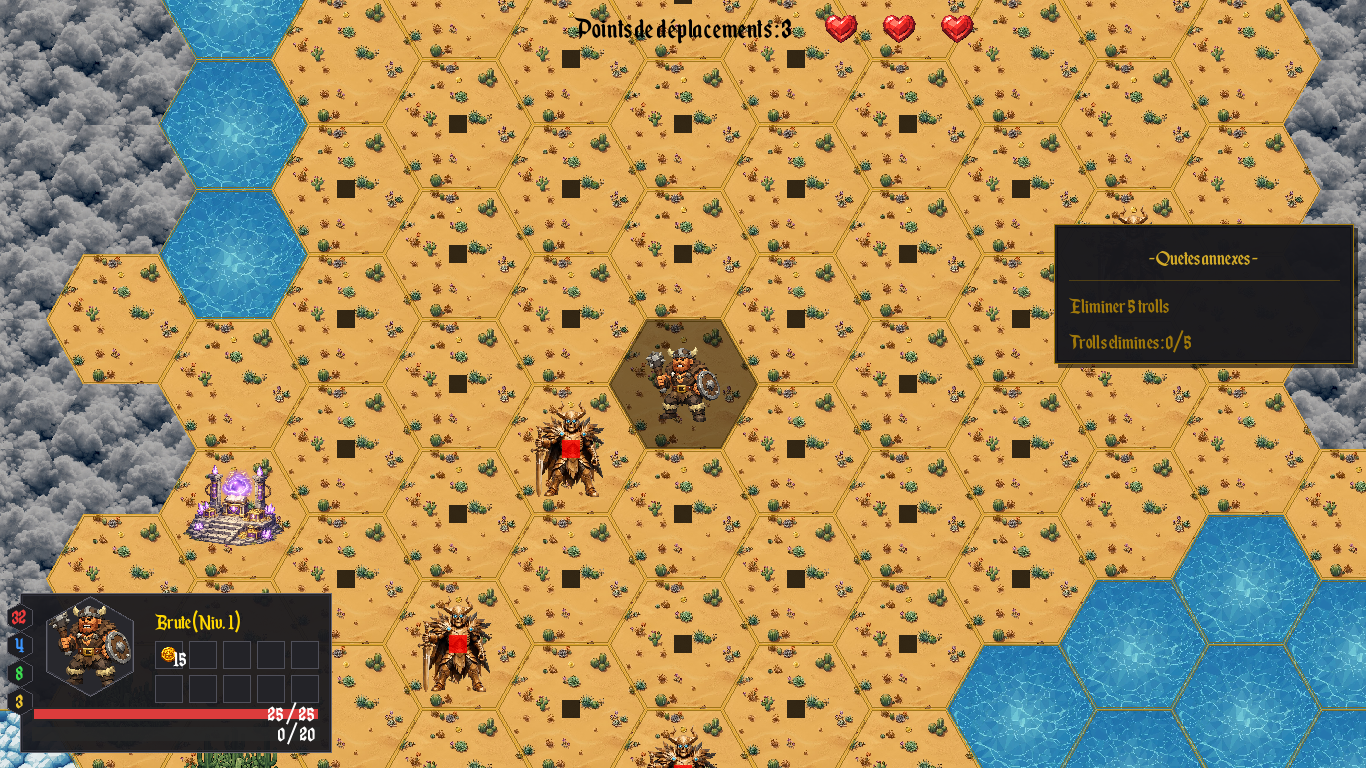
\includegraphics[height=5cm]{carte.png}
\caption{Carte}
\end{figure}

L'ordre du rendu suit les étapes suivantes : dessin des tuiles hexagonales avec leur biome, puis les éléments du décor tels que les obstacles et les bâtiments.
Ensuite, le personnage est affiché par-dessus la carte et, finalement, l'interface utilisateur : barre de vie, barre d'expérience, inventaire, panneaux de quêtes et menus.
Toutes les dimensions et positions sont calculées dynamiquement via SDL2 en fonction de la taille réelle de la fenêtre, ce qui permet au jeu de s'adapter à n'importe quelle résolution sans déformation de l'affichage. 

\subsection{Gestion des combats}

Dans ce jeu, il y a deux types de combat : 
le combat classique effectué avec les différents monstres et le combat final avec le \emph{BOSS\_FINAL}.

L'initialisation du combat se fait via la fonction \emph{creer\_combat}, qui alloue la structure \emph{combat\_t} et lie le personnage au monstre rencontré. 
Les combats sont gérés dans une autre fenêtre que celle de la carte avec la fonction \emph{ouvrir\_fenetre\_combat}. 
Cette dernière charge dynamiquement les textures selon le biome (via \emph{fond\_biome}) et initialise le système audio avec \emph{Mix\_OpenAudio} pour les bruitages d'attaque.
Pour assurer le bon déroulement du combat, les éléments nécessaires sont regroupés dans une structure qui contient :
\begin{itemize}
\item \textbf{Le personnage, le monstre et le tour :} Le tour, géré par \emph{changer\_tour}, identifie l'attaquant actif (\emph{TOUR\_JOUEUR} ou \emph{TOUR\_MONSTRE}).
\item \textbf{L'interface visuelle :} La fenêtre SDL (\emph{pFenetre}) et son moteur de rendu (\emph{renderer}) pour afficher la scène.
\item \textbf{Les textures et polices :} Utilisées pour afficher les informations (du personnage et du monstre) tels que les statisques, le point vie restant et le type du personage et du monstre.
 Les boutons d'action sont rendus via \emph{texture\_attaque\_legere} et \emph{texture\_attaque\_lourde}.
\item \textbf{L'IA décisionnelle :} Pour le monstre, la fonction \sloppy \emph{choix\_attaque\_monstre} analyse les points de vie restants pour décider de la puissance de l'attaque à porter.
\end{itemize}

Une fois le duel terminé, la fonction \emph{combat\_termine} met à jour (gain d'XP, apparition d'une \emph{TOMBE} sur la carte ou état de mort du joueur), puis la fonction \emph{detruire\_combat} libère proprement toutes les ressources mémoire et audio.

\begin{figure}[H]
\centering
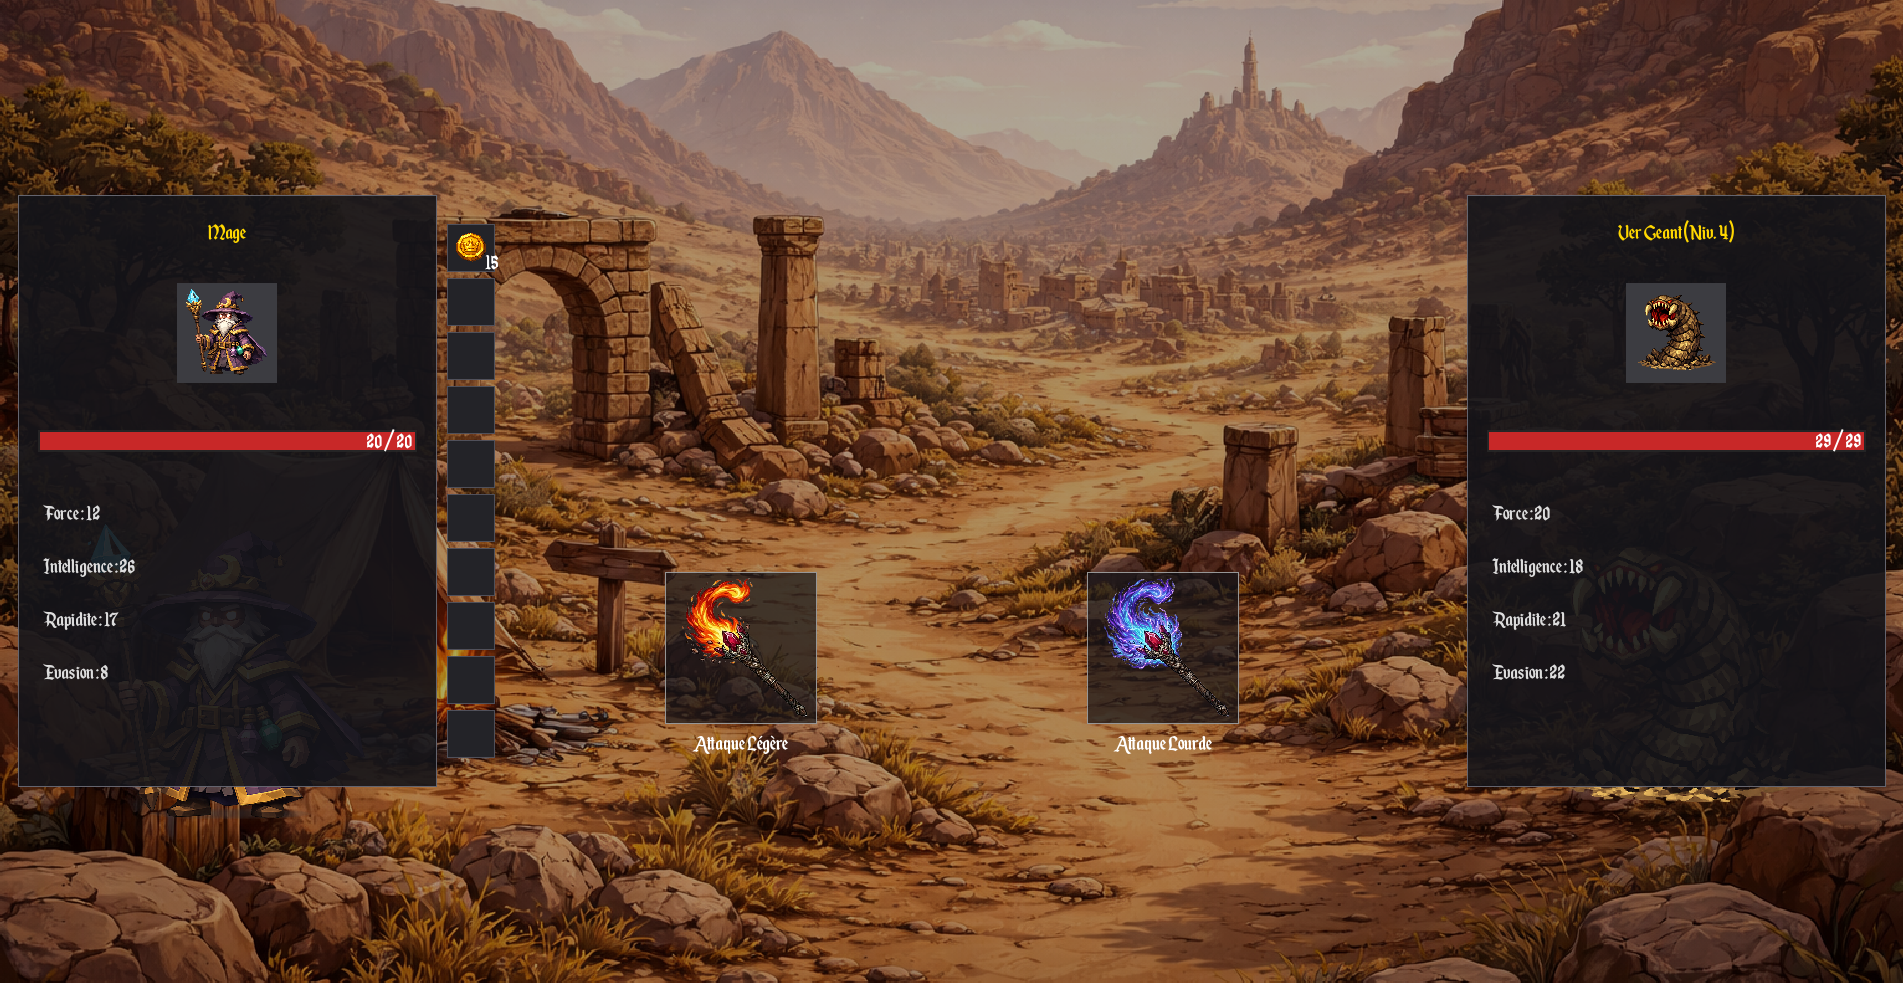
\includegraphics[height=6cm]{../img_jeu/combat_mage.png}
\caption{{\emph{Combat classique}}}
\end{figure}
\hfill
\begin{figure}[H]
\centering
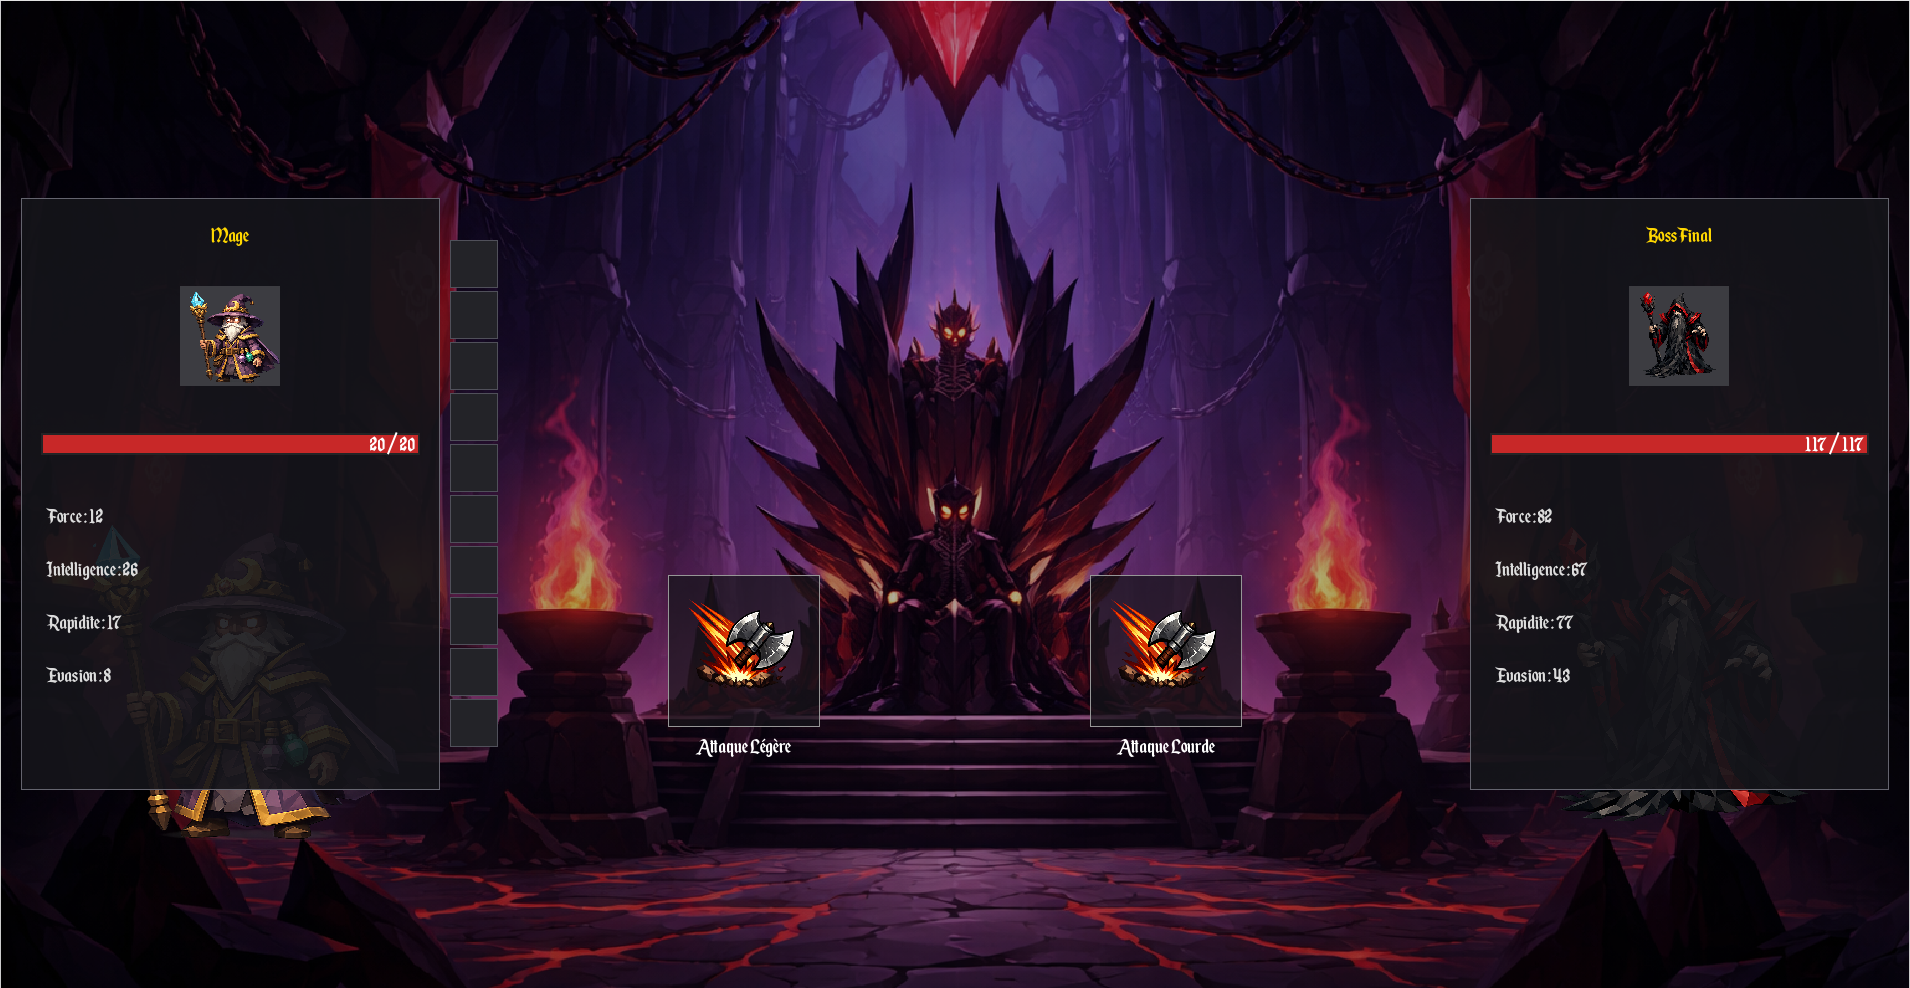
\includegraphics[height=6cm]{../img_jeu/combat_final.png}
\caption{{\emph{Combat avec le boss final}}}
\end{figure}
\newpage

\subsection{Gestion du menu}


Le menu est le premier élément avec lequel le joueur entre en contact. Au lieu d'un simple menu statique, nous avons choisi une approche centrée sur l'UI/UX (User Interface / User Experience) afin de garantir une navigation intuitive, fluide et cohérente avec le style artistique du jeu.

\begin{figure}[h]
\centering
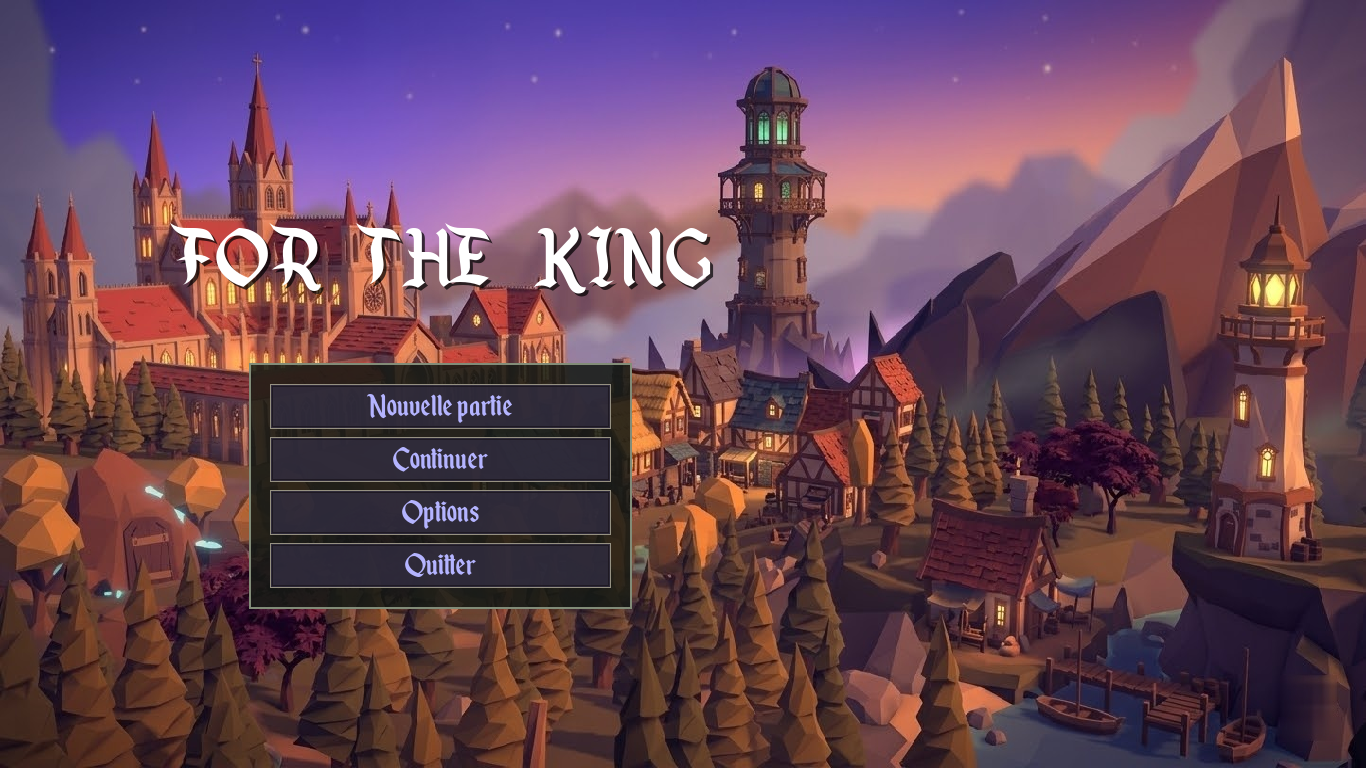
\includegraphics[height=5cm]{menu.png}
\caption{Page principale menu}
\end{figure}

\medskip
\textbf{Mécanique visuelle et interaction} \\
L'interface repose sur une boucle de rendu continue qui gère les interactions de manière dynamique :
\begin{itemize}
    \item \textbf{Détection de survol et retour visuel :} À chaque itération de la boucle, la position de la souris est récupérée via \emph{SDL\_GetMouseState}. La fonction \emph{SDL\_PointInRect} permet de vérifier si le curseur survole un bouton (hitbox). Si c'est le cas, les couleurs de rendu (fond et bordures) sont modifiées en temps réel, offrant un retour visuel intuitif au joueur.
    \item \textbf{Animations :} Lors de la sélection d'un personnage, un effet de "flash" blanc est calculé dynamiquement grâce à la fonction \emph{SDL\_GetTicks}, faisant diminuer l'opacité (\emph{alpha}) sur une durée de 300 millisecondes pour marquer le clic.
    \item \textbf{Gestion Audio :} Un système de fondu enchaîné (\emph{crossfade}) est mis en place avec \emph{Mix\_FadeOutMusic} et \emph{Mix\_FadeInMusic}. Le programme surveille le temps écoulé pour enchaîner deux pistes musicales en boucle sans coupure brutale.
\end{itemize}


\medskip
\textbf{Machine à états et lancement} \\

Le déroulement du menu est géré par une machine à états (les états \emph{ETAT\_PRINCIPAL} et \emph{ETAT\_SELECTION\_PERSO}), ce qui permet d'afficher différents panneaux et logiques sans recharger la fenêtre. 
Une fois que l'utilisateur valide ses choix, le menu prépare le lancement du jeu :
\begin{itemize}
	\item \textbf{Nouvelle aventure} : Le joueur alterne entre les différentes classes de personnages (Mage, Assassin, Brute, Chasseur). Lors de la confirmation, le menu prépare une commande système incluant l'argument \emph{--classe} suivi de la classe sélectionnée, puis lance le jeu.
	\item \textbf{Continuer} : Le menu prépare la commande système avec l'argument \emph{--charger-sauvegarde}.
	\item \textbf{Options} : Un panneau permet d'ajuster le volume général, de basculer en mode plein écran, et d'afficher les commandes (générées dynamiquement avec des encadrés imitant des touches de clavier).
\end{itemize}

\begin{figure}[h]
\centering
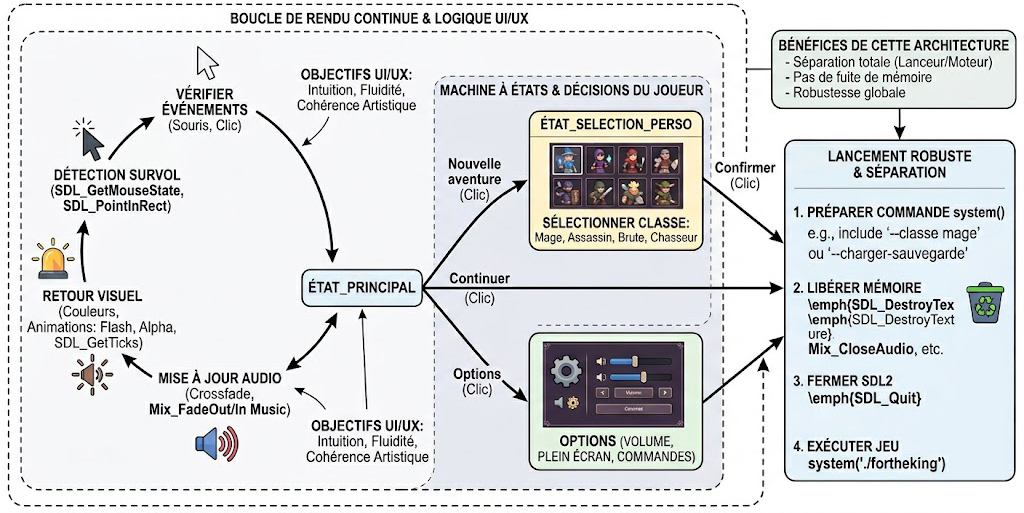
\includegraphics[height=5cm]{menu_schema.jpeg}
\caption{Schéma fonctionnement menu}
\end{figure}

Pour finaliser la transition, le menu libère proprement toute la mémoire allouée avec \emph{SDL\_DestroyTexture} et ferme SDL2 avec \emph{SDL\_Quit}, puis exécute la commande finale via la fonction \emph{system()}. Cela lance l'exécutable principal du jeu (\emph{fortheking}), garantissant une séparation totale entre l'interface d'accueil et le moteur du jeu. Cela permet ainsi d'éviter toute fuite de mémoire et de rendre le programme robuste.

\subsection{Gestion du personnage}


Un personnage est défini par son type (\emph{BRUTE, CHASSEUR, ASSASIN et MAGE}) qui est de type énuméré.
Chaque personnage possède des caractèristiques qui varient selon le type de personnage. Ces caractèristiques sont regroupés dans une structure qui permet de réprésenter le personnage.
Le fonctionnement du personnage repose sur plusieurs étapes :

\begin{itemize}
\item \textbf{Initialisation et typage :}
Le personnage est créé et configuré via la fonction \emph{init\_perso}. Cette fonction alloue la mémoire, 
définit les coordonnées de départ et applique un switch sur le type choisi pour attribuer les statistiques de base (force, intelligence, etc.) propres à chaque personnage.

\item \textbf{Position sur la carte :}
\begin{description}
\item Les coordonnées du personnage, représentées par deux entiers \emph{x} et \emph{y}, permettent de connaître la position du joueur sur la carte. 
Ensuite, la fonction \emph{afficher\_personnage} transforme ces coordonnées en pixels pour dessiner le joueur au bon endroit sur l'écran et s'assure que la vue reste bien centrée sur lui.
\end{description}

\item \textbf{Statistiques et combat :}
\begin{description}
\item Des entiers représentent les dégâts, la force, la santé actuelle (\emph{sante}), le maximum de points de vie (\emph{sante\_max}), l'intelligence, 
la rapidité et le pourcentage d'éviter un coup (\emph{evasion}).
En combat, ces valeurs sont utilisées par des fonctions comme \emph{attaque\_legere} ou \emph{attaque\_lourde} pour calculer l'issue du combat.
\end{description}

\item \textbf{Gestion des tours et progression :}
\begin{description}
\item \textbf{Déplacements :} Le joueur possède des points de déplacements (\emph{pts\_deplacements}). À chaque mouvement, ces points sont décrémentés. 
La fonction \emph{restaurer\_points\_deplacements} est appelée à chaque début de tour pour réinitialiser ces points de façon aléatoire selon la classe. 
La valeur actuelle peut être consultée via \emph{get\_pers\_movements\_points}.
\item \textbf{Progression :} Le niveau évolue avec l'expérience accumulée (\emph{exp}). En cas de victoire, la fonction \emph{monstre\_tue} (appelée dans \emph{combat\_termine}) gère l'attribution de l'expérience et l'incrémentation du compteur \emph{nb\_victime}.
\item \textbf{Économie :} La variable \emph{pieces} permet l'achat d'objets dans l'inventaire, lequel est initialisé par \emph{initialiser\_inventaire} lors de la création du personnage.
\end{description}

\item \textbf{Libération de la mémoire :}
Lorsque la partie se termine ou que le personnage a perdu, la fonction \emph{detruire\_perso} assure la libération de la structure et de son inventaire associé pour éviter toute fuite mémoire.
\end{itemize}

\begin{figure}[H]
\centering
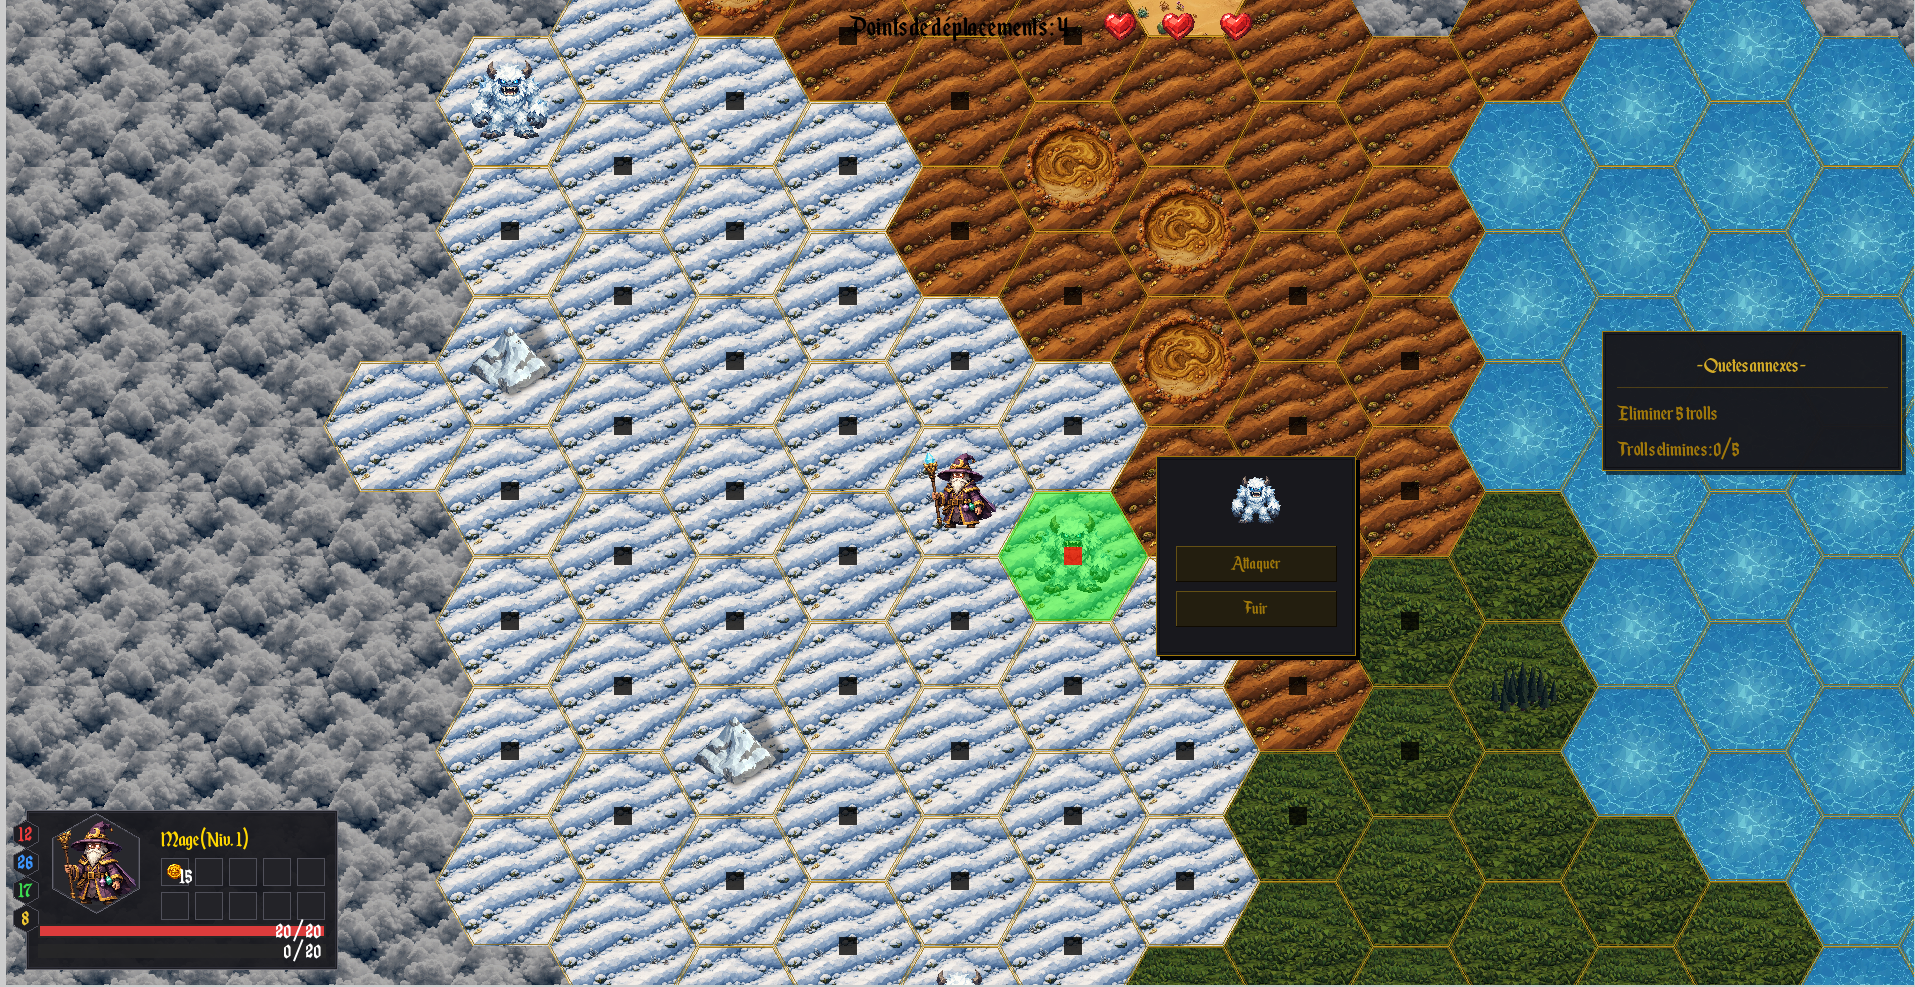
\includegraphics[height=6cm]{../img_jeu/interaction_monstre4.png}
\caption{{\emph{Intéraction du personnage avec un monstre}}}
\end{figure}

\begin{figure}[H]
\centering
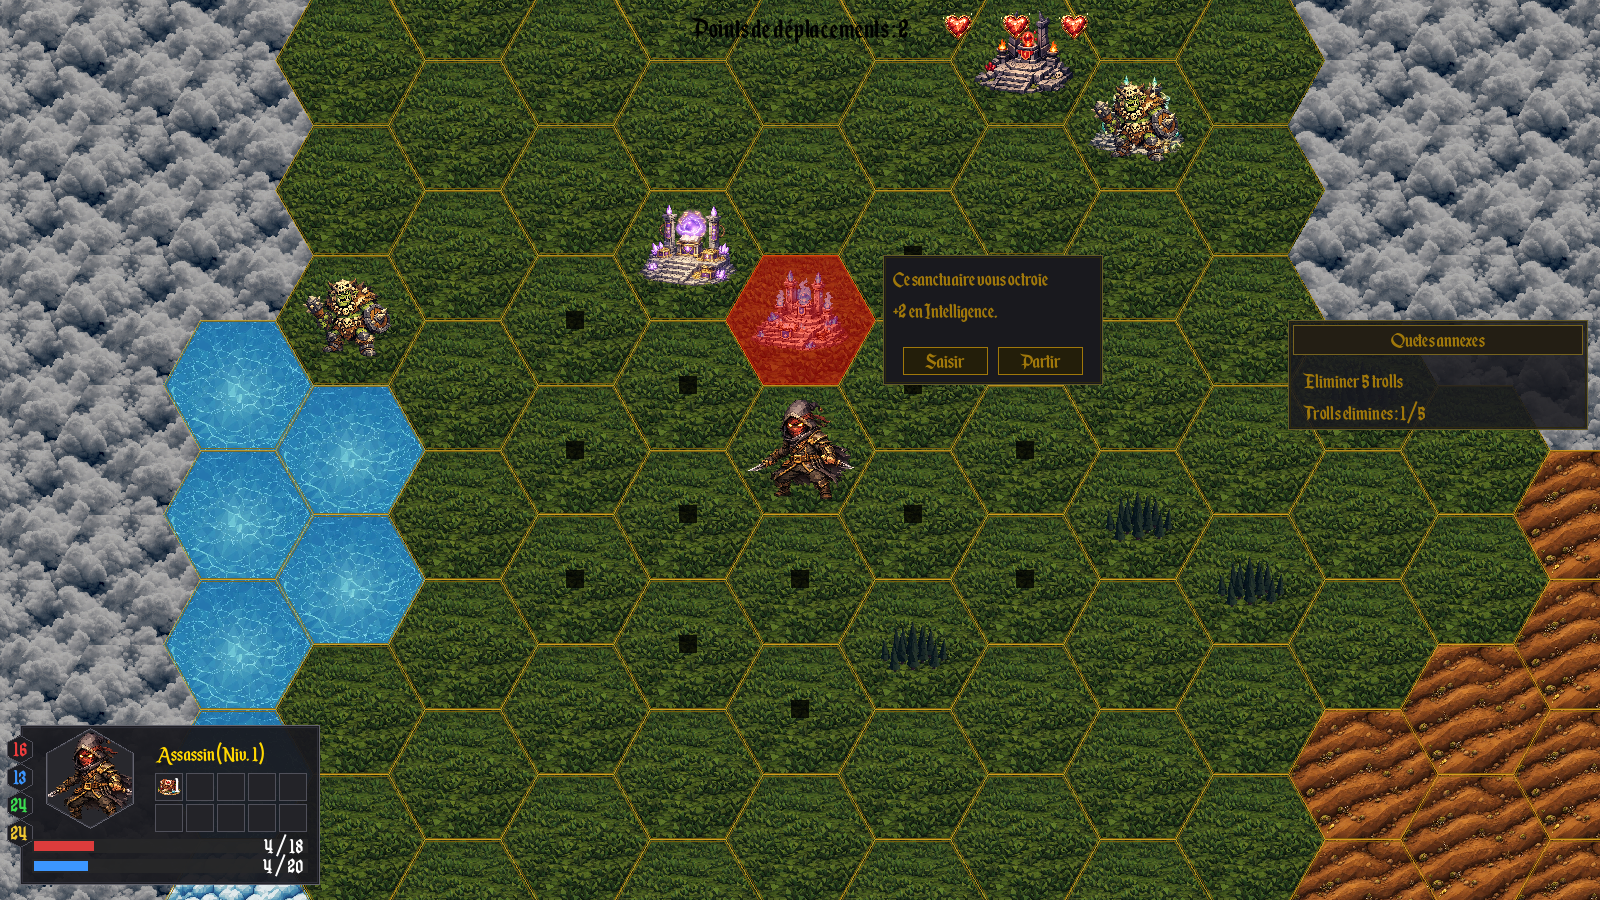
\includegraphics[height=6cm]{../img_jeu/interaction_sanctuaire1.png}
\caption{{\emph{Intéraction du personnage avec un sanctuaire}}}
\end{figure}


\subsection{Gestion de la sauvegarde}

Avant que le programme se termine, une sauvegarde de la partie est effectuée.
Il est donc conseillé de terminer le programme proprement, en appuyant sur le bouton "Quitter" du menu principal.
Cette sauvegarde contient les données du personnage, ainsi que la carte et les différents bâtiments et monstres qui se trouvent sur chaque case.
Lorsqu'on relance le jeu à nouveau, et qu'on appuie sur le bouton "Continuer", le jeu charge la dernière et unique sauvegarde.
Au lieu de générer une nouvelle carte, le jeu va récupérer les informations de l'ancienne partie.
Les sauvegardes sont stockées dans un fichier .txt sous format binaire.
A chaque sauvegarde, on écrase l'ancien fichier, et donc le nouveau fichier commence vide.
D'abord, il faut sauvegarder la carte.
Comme chaque case a les mêmes attributs et la même structure en mémoire, la sauvegarde de la carte devient simple.
Il suffit de faire une boucle sur toutes les cases de la carte et de stocker dans le fichier tous les attributs à la suite.

\section{Bilan et résultats}

Le bilan de notre projet est assez positif.
En effet, les fonctionnalités principales de notre jeu ont été réalisées.
Malgré tout, plusieurs fonctionnalités secondaires n'ont pas pu être implementé, comme par exemple les équipements qui augmentent les statistiques du joueur.
Le planning prévisionnel quant à lui n'a pas été entièrement respecté.
D'abord, nous avons souvent pris du retard sur certaines tâches à faire.
De plus, nous sommes parfois revenus sur des fonctionnalités précédemment implémentées pour les améliorer ou les modifier.
Les raisons qui pourraient expliquer cela sont tout d'abord des bugs imprévus qui retardent le développement, mais également une mauvaise planification initiale des tâches et de leur durée.
Pour améliorer notre projet, si on devait le continuer, on pourrait améliorer les graphismes, rajouter des animations, rajouter des nouveaux objets, monstres, etc.
Ce projet nous a apporté plusieurs choses et compétences intéressantes.
D'abord, il nous a appris une nouvelle compétence technique : l'utilisation de SDL2.
Il nous a également permis de renforcer nos connaissances techniques en algorithmique, et sur les outils techniques comme Git et le débogage.
Concrètement, réaliser ce projet nous a aidé à appliquer les connaissances théoriques vues en cours pour un projet plus "pratique".
Nous avons également appris à organiser, planifier et communiquer correctement pour faire un travail de groupe.
Le projet nous a par exemple familiarisé avec les diagrammes de Gantt pour la planification des tâches.
Il nous a aussi permis de connaître nos limites et comment les surmonter.

\section{Bibliographie}

\begin{thebibliography}{REF}

	\bibitem{Le bruit de Perlin} https://fr.khanacademy.org/computing/computer-programming/programming-natural-simulations/programming-noise/a/perlin-noise
\end{thebibliography}

\newpage

\section{Annexe}

aaaa

\end{document}
